\subsection{Product perspective}

\subsubsection{Scenarios}
It is assumed that in \ref{SCE:user-searches-stations},\ref{SCE:user-books-charge},\ref{SCE:user-pays-charge},\ref{SCE:user-cancels-charge}, \ref{SCE:user-gets-suggestions} the user is already logged in the system (\ref{SCE:user-logs-in})
\begin{enumerate}[label=\textbf{S\arabic*}]
      \item User Signs up:\\
            Lucy, wanting to use the system, opens the app, she is prompted to login or register,
            she chooses to register herself and inserts her personal info (email, password, birthday, payment information, vehicle info);
            an email is sent with a link to confirm the activation of the account, if the link is clicked within
            the first 15 minutes the account is activated and the sign up is successful,
            otherwise it is considered failed and the process must be repeated.\label{SCE:user-signs-up}
      \item User Logs in:\\
            Jay, after signing up, opens the app and he is prompted to insert his email and password,
            if the given information are correct the login is successful and he obtain access to his account
            and the services of the app, otherwise the login is unsuccessful and it must be repeated.\label{SCE:user-logs-in}
      \item User searches for stations:\\
            Robert, opens the app, inserts the location and the time frame to search for charging stations.
            Once submitted, a list of available charging stations is displayed, the list is ordered by the distance of the station
            from the desired location. Via a menu, Robert can choose to order the stations either via distance, price or charging type (super-fast, fast, normal); He can also set to display unavailable stations and set the maximum distance from the chosen location.\label{SCE:user-searches-stations}
            Robert chooses a station and obtains more detailed information.
      \item User books a charge:\\
            Jessica, after choosing a station, decides to book a charge in it selecting the timeslot. Station location and booked time frame are displayed and she is asked to confirm the booking via a popup. She receives a confirmation email with the details
            of the charge (Location, time frame, socket id) and a confirmation pin to insert at the station.\label{SCE:user-books-charge}
      \item User pays a charge:\\
            John, after booking a charge, has to pay it before actually performing it. So he selects the wanted charge and proceeds with the payment. After that he receives an email that summarizes the payment details.\label{SCE:user-pays-charge}
      \item User cancels a charge:\\
            Luke, after booking a charge, wants to cancel it. He opens the app, selects the booking he wants to cancel and presses the Cancel button. A popup appear asking confirmation: if it is pressed the booking is removed, the station returns available, a refound is issued and a confirmation email is sent to the user; otherwise the booking is still valid.\label{SCE:user-cancels-charge}
      \item User charges the vehicle:\\
            Mary, after booking a charge, arrives at the station, she parks her vehicle at the designed socket
            and plugs her vehicle in, Mary then inserts the confirmation pin in the socket to start the charge.
            The socket displays on a monitor the status and the finishing time of the charge.
            Once the charge is finished Mary receives a notification of finished charge,
            she gets her vehicle and completes the charge.\label{SCE:user-charges-vehicle}
      \item User gets charging suggestion based on his calendar:\\
            Josh is a very busy man and also an avid google calendar user,
            setting up every event with correct time and location.
            The service accessing his calendar finds the closest available charging station to each vehicle movement,
            it connects to the vehicle while driving and stores the last charge level and once the battery is below fifty percent Josh gets notified
            about the possibility to charge his vehicle in an available time-slot and near his movement.
            Josh liking the idea opens the app and confirms the booking.\label{SCE:user-gets-suggestions}
      \item \ac{CPO} adds stations to the \ac{CPMS}:\\
            Frank, the responsible for a \ac{CPO}, wants to add stations to the \ac{CPMS} in preparation of subscribing to eMall. For each station he has to insert the \ac{API} reference,
            wether to use the \ac{CPMS} automatic source selector or to choose the preferred energy source.\label{SCE:cpo-adds-stations}
            \todo[inline]{Per questi scenario assumiamo che abbia già fatto il login nel CPMS?}
      \item \ac{CPO} subscribes to the system:\\
            Judy, the CEO of a famous \ac{CPO}, wants to subscribe it to eMAll to improve sales.
            She opens the eMall website and selects to sign up, she inserts the name, email, \gls{partita IVA}, a master password and connects the \acp{CPMS} to the site via an \ac{API} reference.\label{SCE:cpo-signs-up}
      \item \ac{CPO} updates settings and strategy about its system:\\
            The sysadmin of a \ac{CPO}, Andy, after logging in with the master password has access to his \ac{CPMS}.
            Here he can change the energy source, create and update maintainer account inserting the ID and password.\label{SCE:cpo-updates-settings}
            \todo[inline]{Abbiamo davvero bisogno di due livelli di gestion? Sysadmin e cpomaintainer? Secondo me possono collassare in cpo maintainer e quindi eliminare questo scenario}
      \item \ac{CPO}maintainer logs into his assigned \ac{CPMS}:\\
            Brett a \ac{CPO} employee wants to access the service, he connects to the \ac{CPMS} and inserts the ID
            and password, if correct he logs in; otherwise the procedure fails and must be repeated.\label{SCE:cpomaintainer-logs-in}
      \item \ac{CPO} maintainer manages his assigned \ac{CPMS}\\
            Lisa, a maintainer at a cpo logs in the service, here she can see the info of each station of the \ac{CPMS} assigned to her.
            For each station she can: check the status(functioning or not), choose the energy source.
            She can monitor the consumes, profitability and the usage of a specified station.\label{SCE:cpomaintainer-manages}
\end{enumerate}

\clearpage
\todo[inline]{- Il CPO registra il suo servizio nel eMSP convalidato da partita IVA\\
      - Il CPO indica all'eMSP l'accesso all'interfaccia del suo/dei suoi \ac{CPMS}\\
      - L'eMSP contatta l'interfaccia del/dei \ac{CPMS} per ottenere info sulle charging stations\\
      - L'utente paga PRIMA della recharge in base alle info del veicolo e solo dopo il pagamento gli viene assegnato un codice di ricarica che l'eMSP comunica al \ac{CPMS} che lo comunica alla chargingStation che lo accetta per ricarica\\
      - In caso di cancellazione viene effettuato rimborso\\
      - Spostare policy energia a livello della charging station\\
      - Inserire possibilità di imporre DSO alla charging station
      - Eliminare strategia pseudo automatica etc..\\
      - CPO deve contenere una COLLEZIONE di CPMS\\
      - eMSP deve avere una collezione di CPO e non di ChargingStations perchè se no non riesce a parlare con i CPMS.
      MODIFICARE L'UML DI CONSEGUENZA}
\subsubsection{UML diagram}
\begin{figure}[h!]
      \begin{center}
            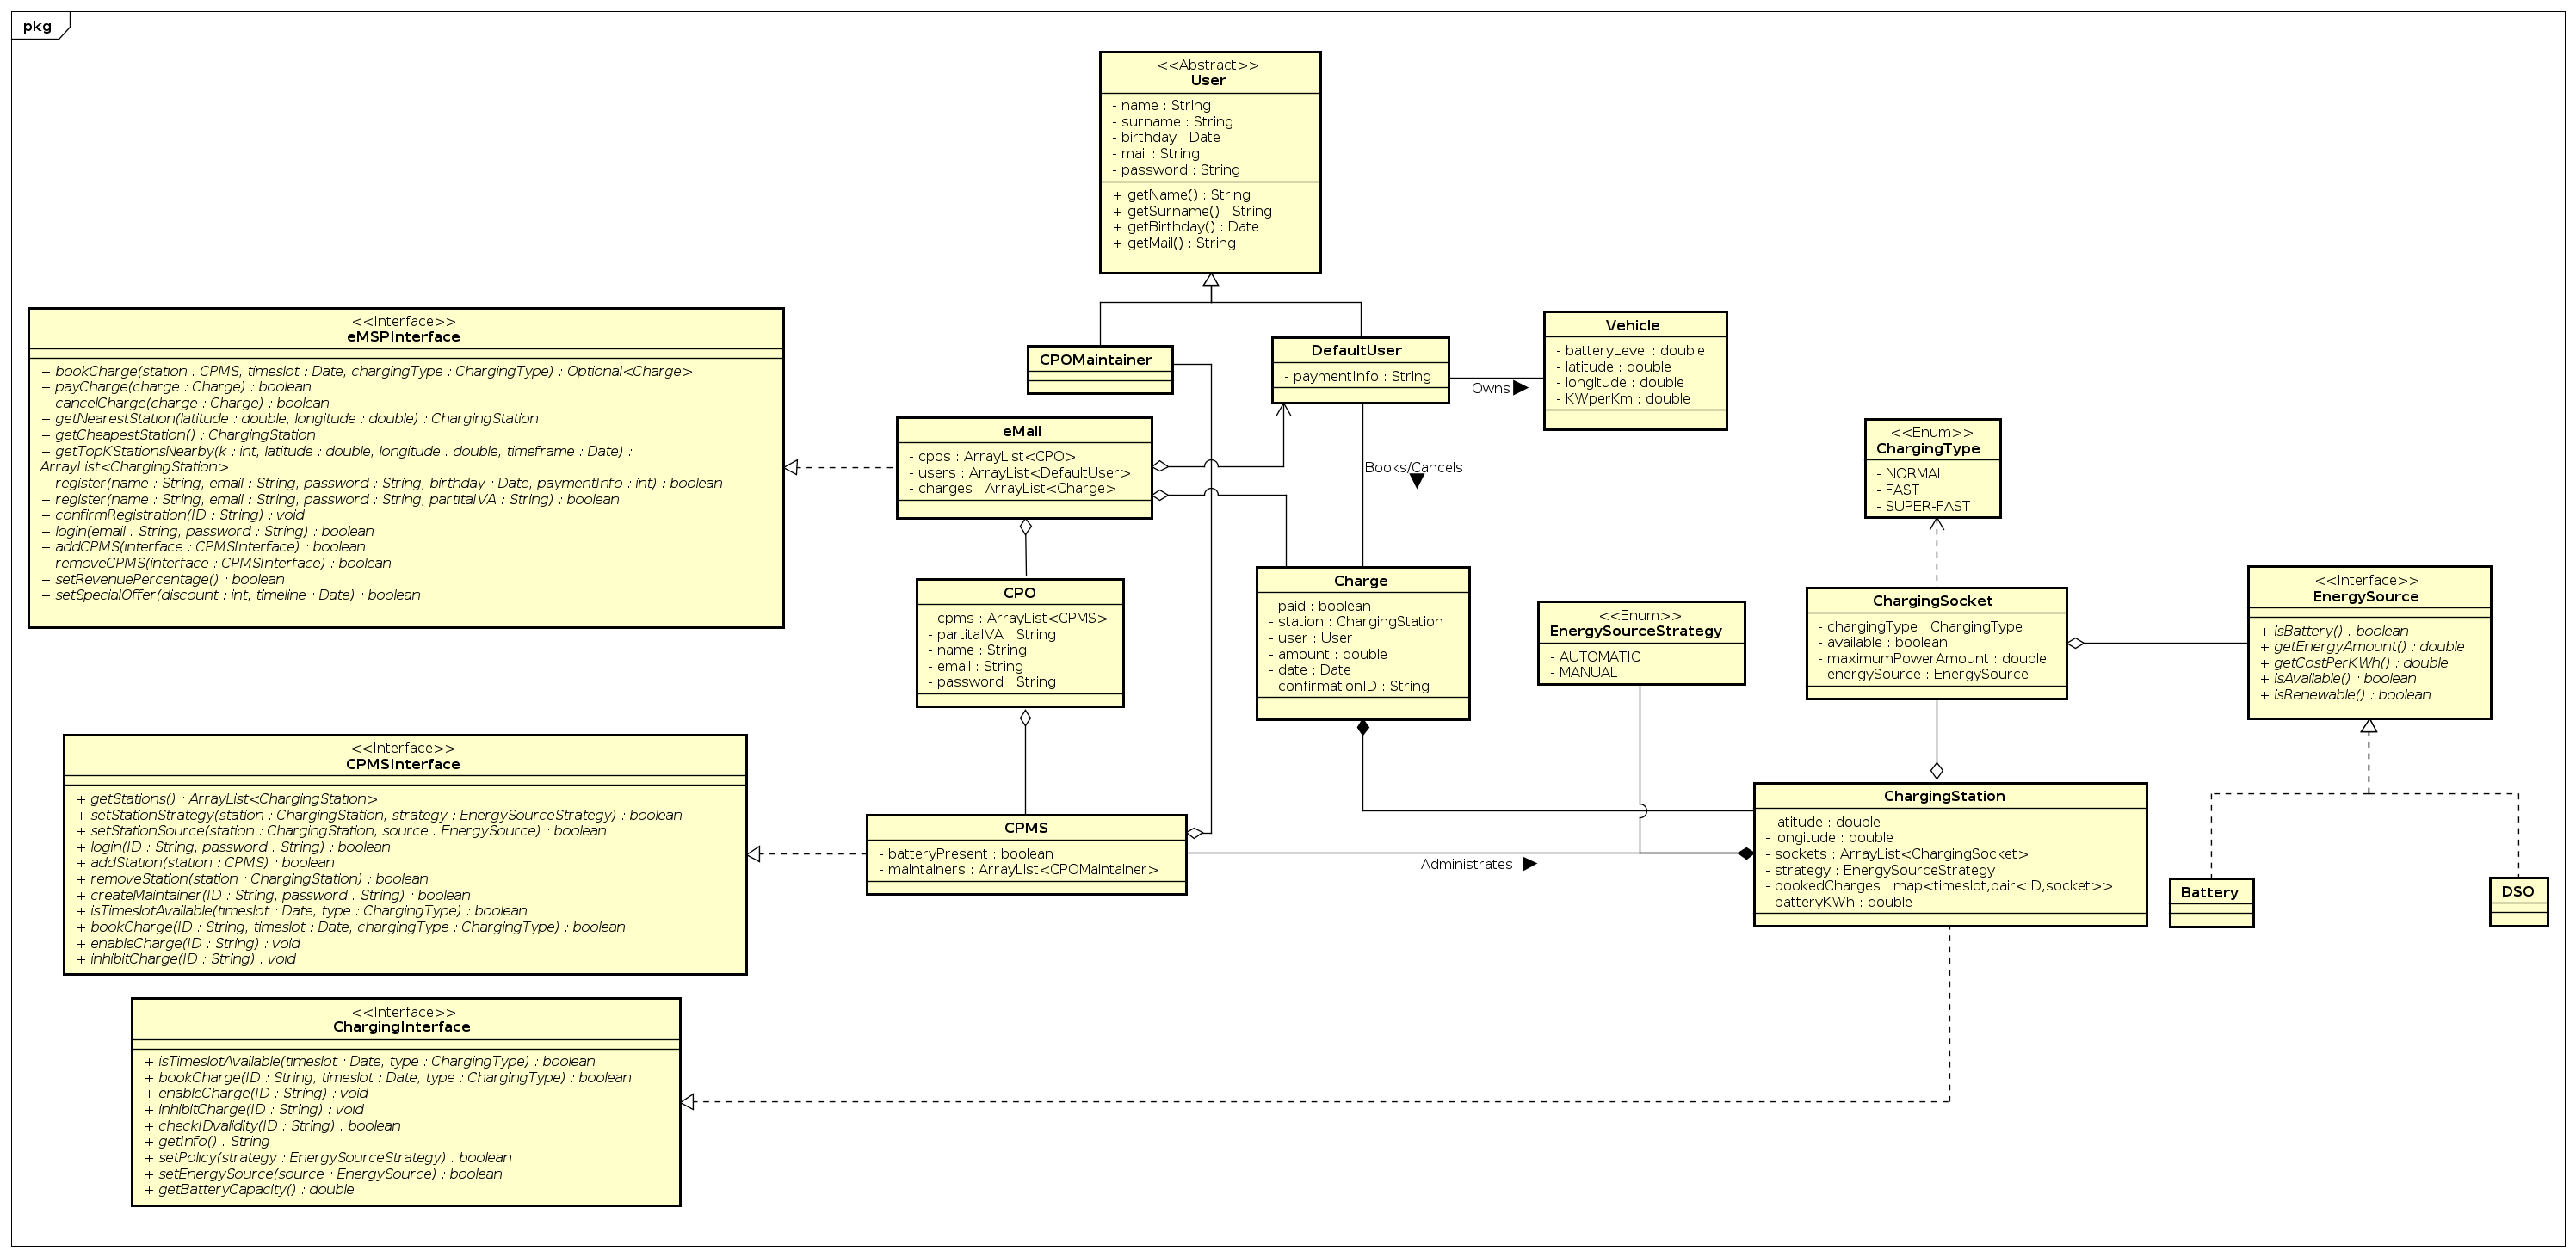
\includegraphics[keepaspectratio, width=16cm]{UML.png}
            \caption{UML}
      \end{center}
\end{figure}

\subsection{Product functions}
In the following subsections the functions of each subsystem are described.

\subsubsection{\ac{eMSP}}
\paragraph{Accessing the \ac{eMSP}}
In order to have features with the usage of personal data (like payment method) the system needs authentication. So a registration and login process is present. When registering it's required to give the system Name, Surname, birthday, e-Mail, Password and a Payment Method. For the login, an authentication with e-Mail and password is required.

\paragraph{Performing a charge}
The principal feature of the system is the ability to help the people to plan a charge for their vehicles efficiently. For this, people can see the availability of charging stations and choose where and in which time slot to charge the vehicle.
Also, if a user changes his mind, there is the possibility to delete a previously booked charge with no charge.
When the user arrives in the booked socket of the charging station, he has to insert the pin that the application displays in order to let the charging process begin.
Always through the application, the user is able to pay for the service thanks to the previously setted payment method.
The system also notifies the user when the charging process is completed.

\paragraph{Retrieving informations about charging stations}
Whenever a user selects a charging station, various informations are shown in order to help the user to make a decision on which station to choose. Informations reguard location, price, a parameter on how green the energy provided is, special offers and availability of sockets in the station.

\paragraph{Get suggestions about the recharge of the vehicle}
An additional feature the system offers reguards a proactive suggestion about the recharge of the vehicle. Thanks to the connection of the application with the vehicle and with the electronic calendar, the system is able to suggest to the user where and when to charge the vehicle in order to satisfy certain parameters chosen by the user. These may involve minimizing the cost of the recharge, minimizing the environment impact of our recharge, minimizing the distance from the scheduled appointments.


\subsubsection{\ac{CPMS}}
\paragraph{Accessing the \ac{CPMS} as \ac{CPO}}
In order to manage the \ac{CPMS} an authentication with proper authorization is required. So \acp{CPO} can login to the system with e-Mail and password. The \ac{CPO} has different informations linked to him in the system, like Name, Surname, e-Mail, password, charging stations that he can manage.
\todo[inline]{2FA for CPO? only login so that the registration will be done by the sysadmin (in this case, add this figure in the rest of the document). If not added manually but we accept registration, it should be authorized by a sysadmin or something like that}

\paragraph{Manage the energy source for a charging station}
An authorized \ac{CPO} can manage stations choosing manually how to charge vehicles, so if he wants to use batteries or \ac{DSO}'s energy in base of their cost and environment impact. In base of these decisions, \acp{CPO} can decide the cost of a charge and special offers to increase visibility of the station in order to promote greener solutions.
Whenever the cost of the energy of some \ac{DSO} is parcticulary convenient the \ac{CPO} can also decide to store it in the batteries. If the \ac{CPO} wishes, the \ac{CPMS} can also work in automatic mode, so the system is able to make all the decisions written above.


\subsection{User characteristics}
We consider the following actors in the \ac{eMall} system:
\begin{enumerate}[label=\textbf{A\arabic*}]
      \item \textbf{Unregistered user:} A user that needs to register before accessing all the \ac{eMall} or \ac{CPMS} services;
      \item \textbf{Registered default user:} A user that has access to all the \ac{eMall} features.
            This actor is associated to an electric vehicle and can visualize the nearest stations, book/cancel/pay a charge, visualize the status of a charge and activate the automatic suggestion service based on the agenda;
      \item \textbf{Registered CPO maintainer user:} A user that has access to all the \ac{CPMS} features.
            These features allow the maintainer to configure the \ac{CPMS} depending on the energy source strategy and visualize all charging stations statuses;
\end{enumerate}

\subsection{Assumptions dependencies and constraints}
\subsubsection{Assumptions}
\begin{enumerate}[label=\textbf{DA\arabic*}]
      \item Users insert genuine data in the forms;
      \item Users(Including CPOs) do not use the system with malicious intent;
      \item All the electric vehicles can be charged by all the stations (no incompatibility);
      \item All the user have an active internet and GPS connection always available while using the service;
\end{enumerate}
\subsubsection{Constraint}
\begin{enumerate}[label=\textbf{C\arabic*}]
      \item If a User wants to change the time slot of a charge he is required to cancel and re-book the charge;
\end{enumerate}

\clearpage